\section{Results and Discussion} \label{section:results}
In this chapter are presented some scenarios and tests with extreme value changes to better understand how the market could evolve in the near future and is also very useful to detect flaws in the model.

\subsection{Basic scenario}
The basic scenario is based on the values explained throughout section \ref{section:model}. Figure \ref{fig:adopters} shows an exponential growth of the population of adopters, characterized by a slow
but steady growth in the beginning (year 2020-2027), and a large growth in the end (year 2028-
2040). In figure \ref{fig:adoption-rate} can also be seen the adoption rate with an exponential behavior, especially in the first 15 years. Both results are obviously connected, by the model definition, and this exponential growth is due to the fact that, as seen earlier, most of the factors are in the acceptable conditions "imposed" by the customers after the first 10 years, meaning that after those 10 years (in 2030) the consumers start more easily and frequently purchasing electric vehicles, hence, the exponential growth.

\begin{figure}[htbp]
\centering
\begin{subfigure}{0.55\textwidth}
  \centering
  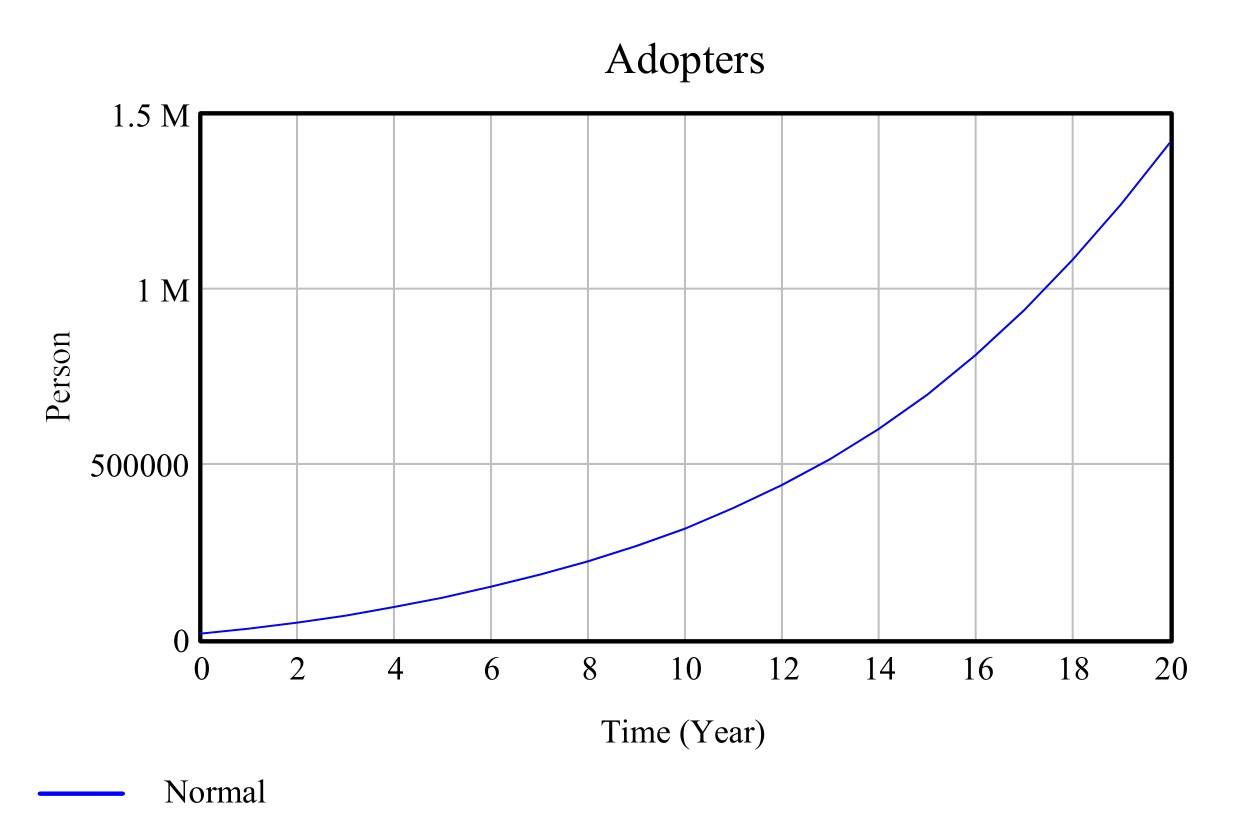
\includegraphics[width=0.98\linewidth]{img/results-basic.jpg}
  \caption{Adopters growth/evolution over the years}
  \label{fig:adopters}
\end{subfigure}%
\begin{subfigure}{0.45\textwidth}
  \centering
  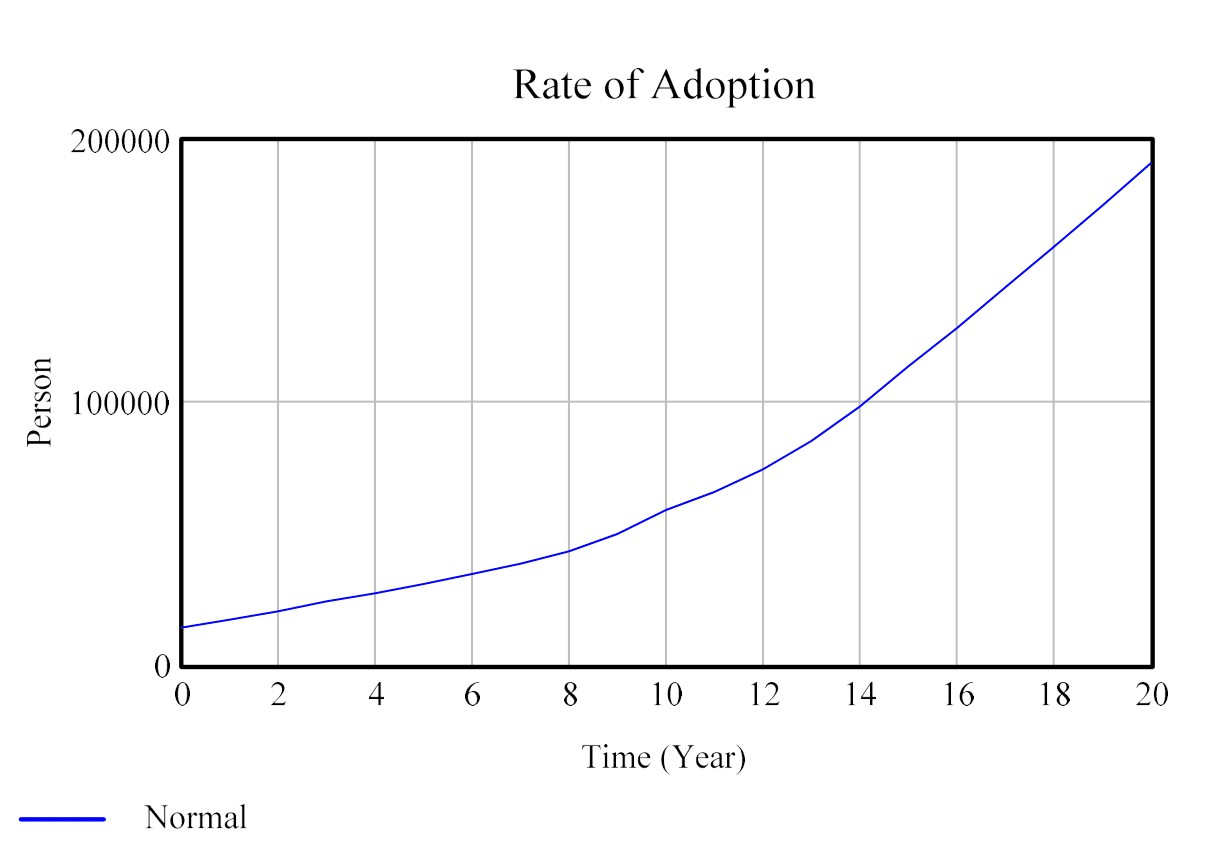
\includegraphics[width=0.98\linewidth]{img/results-basic-adoption-rate.jpg}
  \caption{Rate of Adoption over the years}
  \label{fig:adoption-rate}
\end{subfigure}
\caption{Graphical representation of basic scenario results}
\label{fig:basic-scenario}
\end{figure}

\subsection{Scenario Situations}
Scenario situations use the same values for the model as in the basic situation except from the variable that is being tested or changed to simulate a particular scenario and are useful to create insights for the model and to make the assumptions more reliable.

\subsubsection{Price Difference Effect}
The price difference between an EV and an ICV is the most crucial factor that keeps potential adopters from purchasing an EV. According to the surveys and the information portrayed in section \ref{section:model}, the area around a zero (or negative) price difference has the most effect on the adopters. In contrast to others factors such as driving range, the price difference can be "artificially" influenced through subsidies given by the government. Therefore the subsidy scenario is given in a situation where the government would provide a subsidy of 5000\euro \space on the vehicle fixed price from 2020 to 2029, that is, the first 9 years.

\begin{figure}[htbp]
\centerline{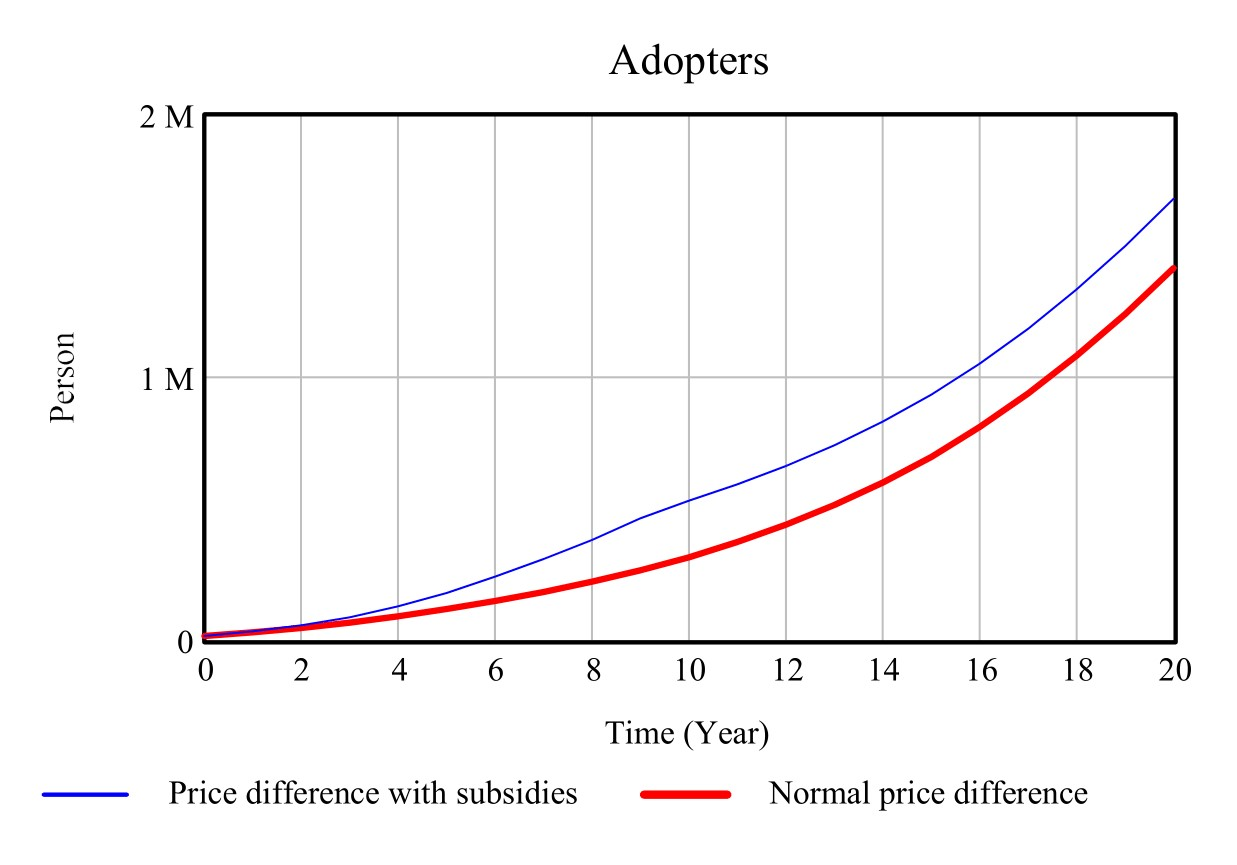
\includegraphics[width=0.7\linewidth]{img/results-price-difference.jpg}}
\caption{Adopters Growth in function of Price Difference variations}
\label{fig:results-price-difference}
\end{figure}

Figure \ref{fig:results-price-difference} shows the result of the scenario described above. As we can see in the graph, the subsidy allowance was effective in the sense that in the first 9 years, the adoption rate clearly increased because in the same time-frame the scenario with the subsidies had a bigger growth of adopters than the basic one. After those 9 years, the adoption rate decreases a little and approximates to the adoption rate of the basic scenario. This "boost" on the first 9 years was able to positively influence the EV market as we ended the 20-year time-frame with considerably more EV adopters in the altered scenario when compared to the basic one. 

\subsubsection{Infrastructure Network Density and Recharge Time Effect}
In this section, the study focuses on the infrastructure network density and the recharge time effects on the EV market.

In this verification, there are 3 different scenarios: \textbf{the normal one}, \textbf{the scenario with a high density infrastructure and slow charging times} and one last \textbf{scenario with a high density infrastructure and fast charging capabilities}. The normal one is the basic scenario referenced earlier.

The other two scenarios have a high density recharging network, meaning that we have total coverage on Portuguese territory from the start (year 2020). The graph of the actual recharge network density in these scenarios has a similar appearance/behaviour to the normal one, being the only difference the starting value that in these scenario has a value of density of 10km, instead of 100km.

What sets these two scenarios apart is the charging times, in one of them, we have slow charging capabilities (with a initial value of 8 hours) and in the other we have fast charging capabilities (with a initial value of 30 minutes).

The time range is set to 10 years, because this better shows the effect of the infrastructure and recharging times in the early phase of the adoption process.

\begin{figure}[htbp]
\centerline{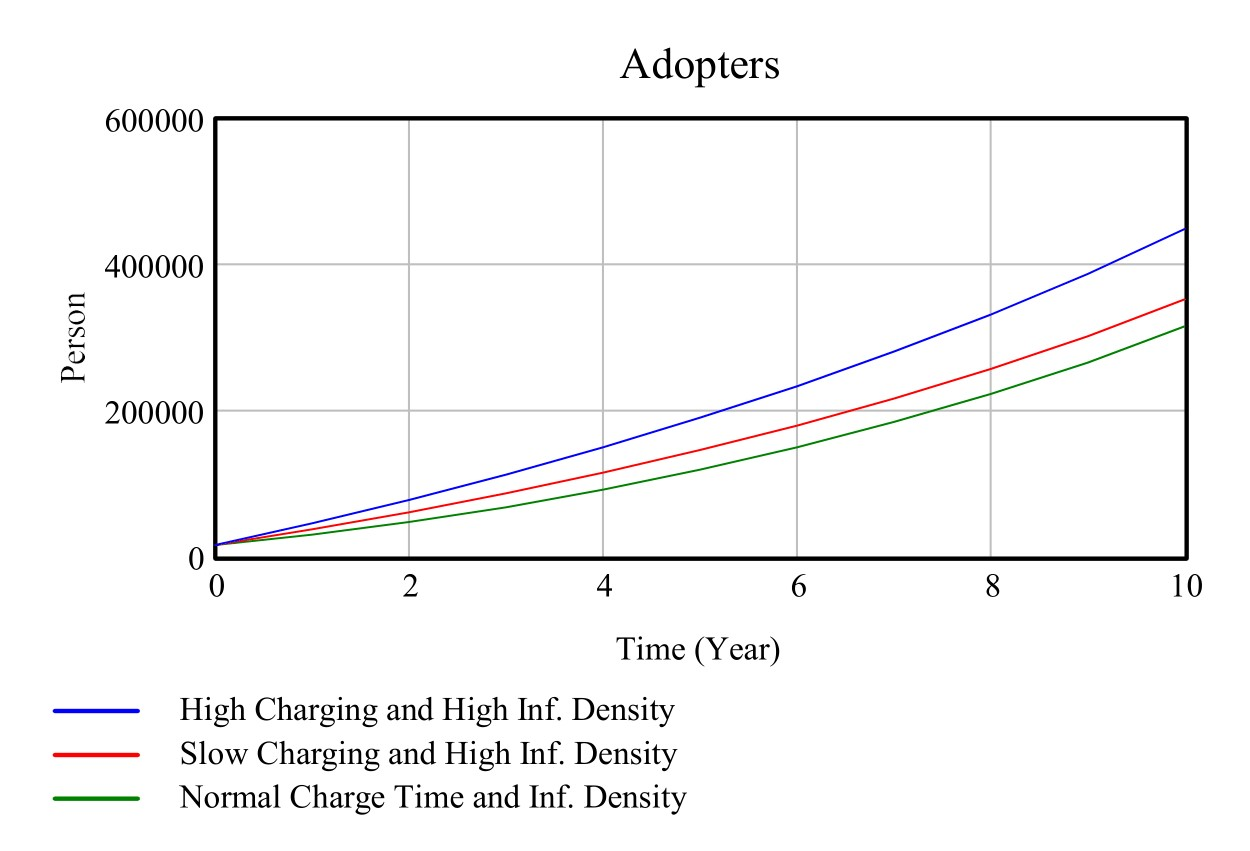
\includegraphics[width=0.7\linewidth]{img/results-time-and-density.jpg}}
\caption{Adopters Growth in function of Infrastructure Density and Charging Time variations}
\label{fig:results-time-and-density}
\end{figure}

Figure \ref{fig:results-time-and-density} shows the result of the scenario described above. As we can see in the graph, these scenario simulations allows us to conclude that the population of adopters increases as result of both \textbf{high infrastructure density} and \textbf{fast charging capabilities}. As we can see, the scenario with high recharge infrastructure density and slow charging is still able to "produce" more adopters than the basic scenario. This is related with the premised stated earlier that a high density recharge network allows for slower charging times, because there is high availability of charging stations. The optimal scenario is when we have a high density charging infrastructure and fast charging capabilities from the start, being these two conditions the best of both worlds. However, a optimistic yet feasible scenario is to have a high density charging network in the early stages of EV introduction (first 10-15 years) and then focusing on improve the charging times of the already existent EV charging stations.

\clearpage